\section{Employee}
\sectionnames{Thanh Tuan Tenh Cong}
\subsection{Concept}
\subparagraph{Description}
In a real world scenario, a company could decide to use the blockchain and the off-chaining approach to verify employee data, which is stored in a private database (RDBMS). Additionally the company wants to make the changes in salaries for each employee as transparent as possible. Together with a union the company can agree on details (e.g. percentage of pay raise, affected departments, etc.) for a pay raise increase and store as well as execute the pay raise on the blockchain.

The general idea behind implementing this use case is to create two separate Smart Contracts: The employee contract and the pay-raise contract. In the employee contract, we need to store the root hashes, which can be used to verify the integrity of employee data records. The details of a pay raise agreed together with a company and a union are stored in a separate contract called the pay raise contract. When performing the pay raise, the employee contract should be addressed which in turn should address the pay raise contract to extract the details for the pay raise.


\textit{Example: A Employees Table}
\begin{center}
    \begin{tabular}{| l | l | l | l | l |}
    \hline
    RecordID & FirstName & LastName & StartDate & Salary \\ \hline
    1 & Max & Mustermann & 20171230 & 45500 \\ \hline
    ... & ... & ... & ... & ... \\ \hline
    \end{tabular}
\end{center}

As mentioned before, the Employee smart contract stores the root hashes of each employee record. The table above shows an example Employee table with one record. The merkle tree is constructed with the values in 'FirstName', 'LastName', 'EntryDate' and 'Salary' in the given record. The root of the constructed merkle tree is stored in a map with the 'RecordID' as an identifier for the root hash.

\subsection{Implementation}
\subparagraph{Overview}

\begin{figure}[h]%evtl:[t] [!htbp]
	\centering
	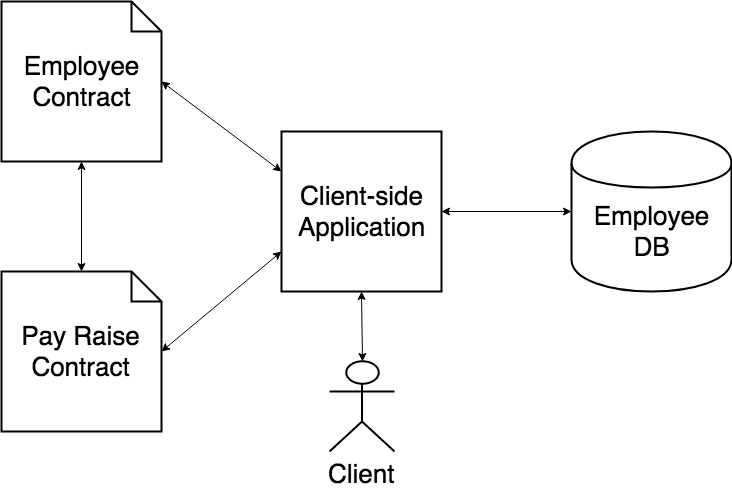
\includegraphics[width=0.8\textwidth]{images/payraiseusecase.png}
	\caption{\label{fig:payraiseusecase}Overview of all components of the Employee Use Case}
\end{figure}

As mentioned in the previous chapter, this use case requires two smart contracts, which should interact with each other. Figure \ref{fig:payraiseusecase} shows all the components of this use case and how they interact with each other. In this use case, we have the following components: Client, Client-side Application, Employee DB, Pay Raise Contract and Employee Contract.

The client is basically the user who is interacting with the whole system. They trigger functions to the client-side application in order to perform transactions. Applied to the use case, the client can be either the company or the union.

The client-side application is the main part of this use case. It is connected with the employee database, where the employee data is stored in an employee table. By using the Web3 API it is able to create and interact with the employee contract as well as the pay raise contract.

Both contracts, the employee contract as well as the pay raise contract, can exist on their own. But only one employee contract should be created for this use case. Everytime data is inserted or updated in the employee database, the employee contract is updated accordingly. E.g. when a record is inserted in the database, an additional mapping item with the identifier and the Merkle root of the Merkle tree constructed from this record is inserted into the contract. In case a record is updated, a new Merkle tree has to be constructed in the client-side application and the new Merkle root has to be used to replace the old Merkle root in the equivalent mapping item.

\subparagraph{Necessary Steps}

This subchapter briefly describes the necessary steps for a client to interact with the components in the use case. Also it gives some insights on how the components interact with each other.

\begin{enumerate}
	\item Create Employee Contract
\end{enumerate}

In order to perform further transactions, an employee contract has to be created. Via REST interface, the client shall call a function to create a contract. The client-side application takes the request and creates the contract in the network as well as a contract instance inside the application with the contract address, to perform further transactions with the employee contract.

\begin{enumerate}[resume]
	\item Create/Import Employee Data
\end{enumerate}

The client can now create data records or use the import function, to create multiple employee data records. The client-side application uses the input of the client to create data records in the employee table in the database. Moreover, it creates a Merkle tree for each new employee record and adds a mapping item with the Merkle root and the “record id” of the employee in the database into the smart contract. 

\begin{enumerate}[resume]
	\item Create Pay Raise Contract
\end{enumerate}

Before a pay raise can be given to employees, specific conditions have to be formulated, for example the percentage, the affected department, etc. Those conditions are formulated in the Pay Raise Contract. This contract contains only the formulated and agreed upon conditions between the company and the union, as well as getter functions to retrieve these conditions later from the Employee Contract, where the pay raise is executed.

\begin{enumerate}[resume]
	\item Increase Salary
\end{enumerate}

In the Increase Salary step, the client triggers a function on the client-side application to increase the salary of all affected employees according to the created pay raise contract in step 3. Therefore the client sends a request with the contract address of the pay raise contract. The client-side application calls a function in the employee contract by passing the pay raise contract as input parameter. After that the employee contract retrieves the conditions (e.g. percentage, department, etc.) from the pay raise contract and returns it to the client-side application as an event. The client-side application listens to this event and uses the conditions as query parameters when querying the database. For example, if the department is ‘IT’, the SQL Query would look like this:

\begin{lstlisting}[language=bash]
SELECT *
FROM Employee
WHERE Department = 'IT'
\end{lstlisting}

For each single employee in the output of the query, a single smart contract transaction is required to increase the salary of the employee. If for example, the number of employees in the IT department is three, then the whole transaction needs three additional smart contract transactions. These three smart contract transactions are chained, meaning they need to be executed sequentially. The reason for that is because the employee contract will send data back to the client-side application via an event. The design decision was to shut down the event listener in the client-side application after it listened to one event. Triggering three smart contract transactions would result in three different events as a result of each transaction. Triggering all three smart contract transactions at once would mean that the client-side application would only listen to one event and the whole transaction cannot be completed.

As a first step in one smart contract transaction for increasing the salary of one single employee, the client-side application calls a smart contract function and sends the whole data record of the employee in the database table as well as the Merkle proofs of the salary of the single employee as input parameters to the smart contract. In the smart contract the integrity of the employee data record is checked. The Merkle root can be retrieved from the mapping item with the record identifier and the Merkle root stored in the smart contract. With the Merkle proof and the hash of the salary of the employee, the Merkle root can be constructed. If the constructed Merkle root is the same as the saved Merkle root for the employee record, the integrity check was successful. The salary is then increased by the percentage stored in the pay raise contract. A new Merkle root is constructed out of the new salary and the proofs, which is then stored into the mapping item and sent back as an event to the client-side application together with the new value of the salary. The client-side application takes the new value of the salary of the employee and stores it into to the database. Subsequently, it will continue to create a new smart contract transaction for the next employee pay raise. The whole transaction is finished when all employees in the query result are processed.

In case the integrity check fails, the smart contract will send an event to notify the client-side application about the failure. Even if one integrity check of an employee fails, the other employees are still processed. The end result is that the client will receive as a response a list of all the employees whose salary have been increased.

\subparagraph{Discussions}

In this use case the client-side application needs to trust the database to return the correct results. For example if there are actually five people working in the IT department, the database should return the records of those five employees. In this case we are putting some trust in the database to return all of those five employees. However,the database could be manipulated by an administrator, so that one or more employees from the IT department are missing in the query result. As a result a pay raise would not affect those missing employees. A possible solution would be to store the number of employees for each department in the smart contract and check whether the number of query results matches the number of employees for a specific department stored in the smart contract.
